\documentclass[10pt]{beamer}

\usepackage{packages}
\title{Exercício Programa 2}
\subtitle{Corrida por eliminação}
\institute{IME-USP}
\author{Lucas Paiolla Forastiere, 11221911\\ Marcos Siolin Martins, 11221709}
\date{05 de novembro de 2020}

\begin{document}
    \maketitle

    \section{Detalhes de Implementação}

    \begin{frame}{Detalhes de Implementação - Os competidores}
        \begin{itemize}
            \justifying
            \item Cada ciclista possui uma \texttt{struct} própria com todas
                as informações necessárias para a corrida e as estatísticas;
            \item Essas \texttt{structs} ficam armazenadas em um vetor global
                chamado \texttt{ciclistas};
            \item Enquanto isso, as threads de cada ciclista ficam em um vetor
                à parte chamado \texttt{threads}.

        \end{itemize}
    \end{frame}

    \begin{frame}{Detalhes de Implementação - A pista}
        \begin{itemize}
            \justifying
            \item A pista é uma matriz de inteiros com tamanho máximo de
                \texttt{D\_MAX (2000)} por \texttt{FAIXAS (10)}. Se
                \texttt{pista[i][j]} é $0$, então não há nenhum ciclista no
                metro $i$, faixa $j$, caso contrário, o número dessa posição é
                o ciclista que se encontra nela;
            \item Além disso, existe uma matriz \texttt{mutex\_pista} de mesmas
              dimensões com um \textit{mutex} para cada posição da pista.
        \end{itemize}
        \textbf{Obs.:} Existe uma constante chamada \texttt{COM\_COR} em
        \texttt{util.c} que, quando alterada para $1$, realiza a depuração da
        pista colorindo os ciclistas na saída.
    \end{frame}

    \begin{frame}{Detalhes de Implementação - O movimento - 1}
      \begin{itemize}
        \justifying
        \item Cada ciclista é responsável por seu próprio movimento, liberando
          ou travando os \textit{mutexes} necessários. Sempre que precisamos
          checar uma posição da pista, travamos o \textit{mutex} correspondente,
          fazemos as verificações e depois o liberamos;
          \item Se a posição da frente está livre, então ele simplesmente anda
          para frente;
        \item Se ela está ocupada por um ciclista que ainda não fez sua ação,
          então esperamos por ele (liberando o seu \textit{mutex});
      \end{itemize}
    \end{frame}

    \begin{frame}{Detalhes de Implementação - O movimento - 2}
      \begin{itemize}
        \justifying
        \item Se ele está a mais que $30$ Km/h e não conseguiu andar para
          frente, então ele tenta ultrapassar (verificando as faixas mais
          externas);
        \item Na verificação, se ele não conseguir travar o
          \textit{mutex} por qualquer motivo, então tenta a próxima faixa mais
          externa.
      \end{itemize}
    \end{frame}

    \begin{frame}{Detalhes de Implementação - Turnos e Barreiras - 1}
      \begin{itemize}
        \justifying
        \item Nós dividimos as interações dos ciclistas em \textbf{turnos}. Cada
          final de turno é protegido por uma barreira, para garantir que todos
          os ciclistas então sincronizados em seus turnos;
        \item Os turnos em que um ciclista se movimenta são definidos de acordo
          com sua velocidade;
        \item Ciclistas a $30$ Km/h se movimentam de $6$ em $6$, enquanto os a
          $60$ se movimentam de $3$ em $3$ e os a $90$, de $2$ em $2$;
        \item Dessa forma, cada \textbf{turno} representa $20$ ms de simulação;
      \end{itemize}
    \end{frame}

    \begin{frame}{Detalhes de Implementação - Turnos e Barreiras - 2}
      \begin{itemize}
        \justifying
      \item Além disso, na barreira, temos uma região que é responsável por
        ações de sincronização, como remover ciclistas eliminados, refazer a
        barreira (pois estamos utilizando a do \texttt{pthread}), incrementar o
        tempo atual da simulação e imprimir a pista caso necessário;
      \item Portanto, não foi necessária uma thread coordenadora, já que os
        próprios ciclistas são responsáveis pela sincronização.
      \end{itemize}
    \end{frame}

    \begin{frame}{Detalhes de Implementação - Linha de Chegada - 1}
      \begin{itemize}
        \justifying
      \item Sempre que um ciclista cruza a linha de chegada, nós verificamos se
        ele precisa ser eliminado, se quebrou ou se já terminou a corrida;
      \item Assim que ele cruza, nós adicionamos ele a uma lista ligada que dá
        as classificações referentes à volta que ele acabou de completar. Assim
        sabemos volta a volta as classificações;
      \item Além disso, existe uma outra lista ligada referente a quantos
        ciclistas quebraram em uma determinada volta. Caso ele quebre,
        adicionamos ele na lista ligada daquela volta;
      \end{itemize}
    \end{frame}

    \begin{frame}{Detalhes de Implementação - Linha de Chegada - 2}
      \begin{itemize}
        \justifying
      \item Para eliminar um ciclista, nós mantemos uma variável \texttt{ult}
        referente à volta posterior à última completa. Assim sendo, quando
        \texttt{ult} é uma volta par, devemos eliminar o último a completá-la;

      \item Quando um determinado ciclista está completando sua
        \texttt{ult}-ésima volta, devemos verificar se a volta \texttt{ult}
        terminou (isto é, se todos os ciclistas já a completaram);

      \item Para saber se ela está completa, verificamos se o número de
        ciclistas que já completaram \texttt{ult} menos o número de ciclistas
        que quebraram em \texttt{ult} é igual ao número de ciclistas que
        completaram \texttt{ult-1}, menos 1 caso \texttt{ult-1} seja uma volta
        par, isto é, alguém foi eliminado;
      \end{itemize}
    \end{frame}

    \begin{frame}{Detalhes de Implementação - Linha de Chegada - 3}
      \begin{itemize}
        \justifying
      \item Quando detectamos que a volta \texttt{ult} foi completada, devemos
        imprimir seu ranking e verificar se alguém deve ser eliminado;
      \item Se sim, então marcamos o último ciclista a passar por \texttt{ult}
        como eliminado nessa volta e precisamos verificar agora se a volta
        \texttt{ult+1} também já está completa (caso o último a passar
        pela volta \texttt{ult} estiver \textit{muito} atrás na corrida);
      \end{itemize}
    \end{frame}

  \begin{frame}{Detalhes de Implementação - Linha de Chegada - 4}
      \begin{itemize}
        \justifying
      \item Por fim, precisamos mudar as velocidades dos ciclistas. Para as
        velocidades $30$ e $60$ Km/h é fácil, basta fazer como pedido no
        enunciado;
      \item Já para determinar se alguém estará a $90$ Km/h, precisamos prever
        que determinado ciclista está nas duas últimas voltas;
      \item Para fazer isso, nós mantemos a variável global \texttt{max\_voltas},
        que é dada pela fórmula $\texttt{max\_voltas} = \texttt{ult} + 2 *
        (n_{ult}-1)$, onde $n_{ult}$ é a quantidade de ciclistas que passaram
        para a volta \texttt{ult+1};
      \item Com ela, nós sabemos exatamente quantas voltas a corrida terá caso
        todos que estão correndo não quebrem e, assim, conseguimos determinar se
        alguém está nas duas últimas voltas;
      \end{itemize}
    \end{frame}

    \begin{frame}{Detalhes de Implementação - Linha de Chegada - 5}
      \begin{itemize}
        \item Para decidir se haverá alguém correndo a $90$ Km/h, realizamos um
          teste no início do programa usando a probabilidade de $10\%$;
        \item Caso um ciclista comece a correr a $90$ Km/h, mas já deveria ser
          eliminado em uma volta anterior, então, ao ser eliminado, o próximo
          que entrar nas duas últimas voltas, correrá a $90$ Km/h.
      \end{itemize}
    \end{frame}


    \section{Testes}
    \subsection{Medições}
    \begin{frame}{Realização das Medições}
      \begin{itemize}
        \item Para medir tempo consumido, usamos o comando \texttt{time} do
          bash;
        \item Para medir a memória consumida usamos o comando \texttt{pmap}
          passando o \textit{PID} do processo.
      \end{itemize}
      Os resultados que obtivemos foram os seguintes:
    \end{frame}

    \subsection{Experimentos}
    \begin{frame}{Quantidade Normal de Ciclistas - Tempo}
        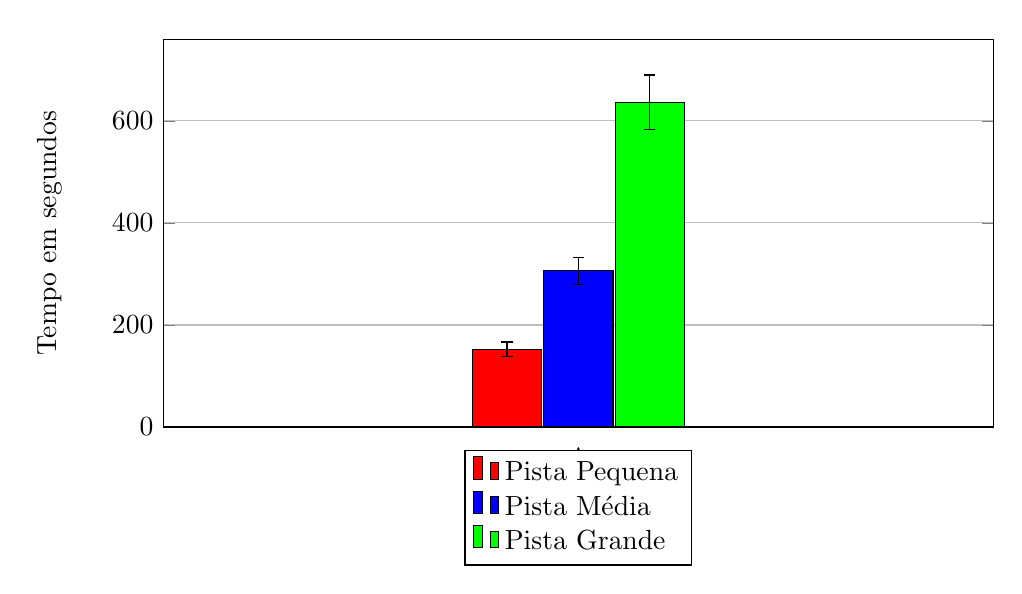
\begin{tikzpicture}
              \begin{axis}[
                  width  = 1.00*\textwidth,
                  height = 6.5cm,
                  major x tick style = transparent,
                  ybar=2*\pgflinewidth,
                  bar width=25pt,
                  ymajorgrids = true,
                  symbolic x coords={A},
                  xtick = data,
                  scaled y ticks = false,
                  enlarge x limits=0.50,
                  ymin=0,
                  ylabel={Tempo em segundos},
                  ylabel style={yshift=0.4cm},
                  legend cell align=left,
                  legend style={at={(0.5,-0.06)},anchor=north},
              ]

              \addplot[style={fill=red},
                error bars/.cd,
                y dir=both,
                y explicit]
              coordinates {
                  (A, 152.6) += (0,14.01) -= (0,14.01)
              };

              \addplot[style={fill=blue},
                error bars/.cd,
                y dir=both,
                y explicit]
              coordinates {
                  (A, 306.2) += (0,26.32) -= (0,26.32)
              };

              \addplot[style={fill=green},
                error bars/.cd,
                y dir=both,
                y explicit]
              coordinates {
                  (A, 636.76) += (0,53.16) -= (0,53.16)
              };

              \legend{Pista Pequena, Pista Média, Pista Grande}

            \end{axis}
        \end{tikzpicture}
    \end{frame}

    \begin{frame}{Quantidade Normal de Ciclistas - Memória}
        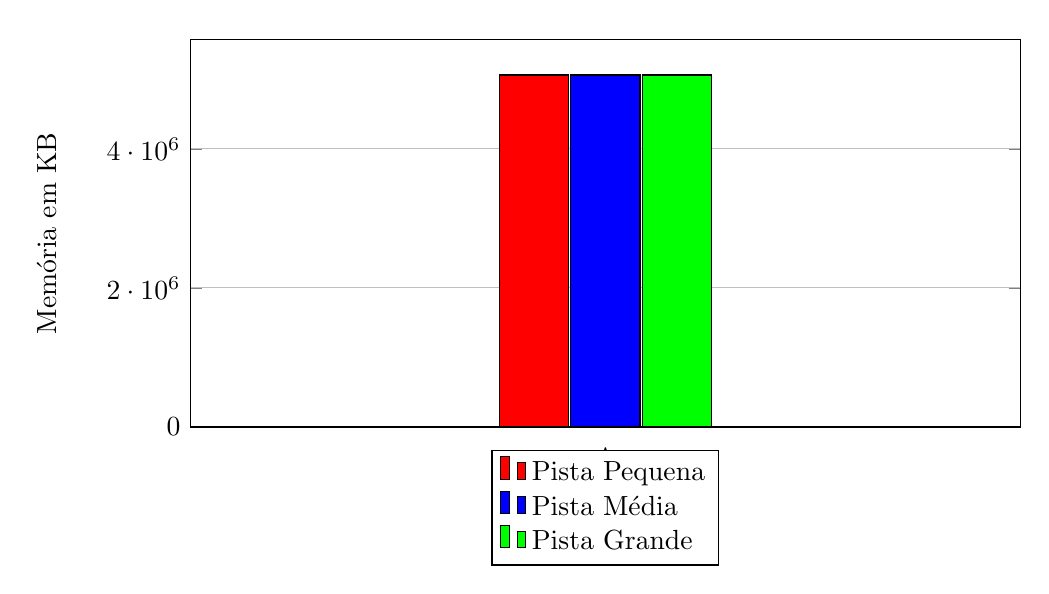
\begin{tikzpicture}
              \begin{axis}[
                  width  = 1.00*\textwidth,
                  height = 6.5cm,
                  major x tick style = transparent,
                  ybar=2*\pgflinewidth,
                  bar width=25pt,
                  ymajorgrids = true,
                  symbolic x coords={A},
                  xtick = data,
                  scaled y ticks = false,
                  enlarge x limits=0.50,
                  ymin=0,
                  ylabel={Memória em KB},
                  ylabel style={yshift=0.4cm},
                  legend cell align=left,
                  legend style={at={(0.5,-0.06)},anchor=north},
              ]

              \addplot[style={fill=red},
                error bars/.cd,
                y dir=both,
                y explicit]
              coordinates {
                (A, 5061693.33)
              };

              \addplot[style={fill=blue},
                error bars/.cd,
                y dir=both,
                y explicit]
              coordinates {
                (A, 5061693.33)
              };

              \addplot[style={fill=green},
                error bars/.cd,
                y dir=both,
                y explicit]
              coordinates {
                (A, 5061693.33)
              };

              \legend{Pista Pequena, Pista Média, Pista Grande}

            \end{axis}
        \end{tikzpicture}
    \end{frame}

    \begin{frame}[label={segs}]
      \frametitle{Tamanho Normal de Pista - Tempo}
        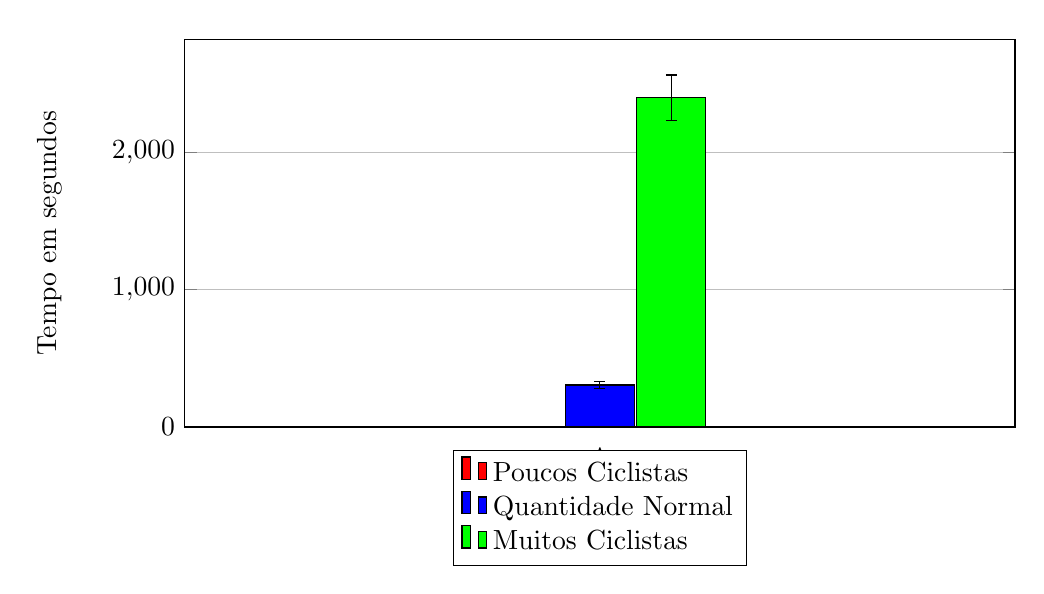
\begin{tikzpicture}
              \begin{axis}[
                  width  = 1.00*\textwidth,
                  height = 6.5cm,
                  major x tick style = transparent,
                  ybar=2*\pgflinewidth,
                  bar width=25pt,
                  ymajorgrids = true,
                  symbolic x coords={A},
                  xtick = data,
                  scaled y ticks = false,
                  enlarge x limits=0.50,
                  ymin=0,
                  ylabel={Tempo em segundos},
                  ylabel style={yshift=0.4cm},
                  legend cell align=left,
                  legend style={at={(0.5,-0.06)},anchor=north},
              ]

              \addplot[style={fill=red},
                error bars/.cd,
                y dir=both,
                y explicit]
              coordinates {
                (A, 0.5) += (0,0.29) -= (0,0.29)
              };

              \addplot[style={fill=blue},
                error bars/.cd,
                y dir=both,
                y explicit]
              coordinates {
                  (A, 306.26) += (0,26.32) -= (0,26.32)
              };

              \addplot[style={fill=green},
                error bars/.cd,
                y dir=both,
                y explicit]
              coordinates {
                  (A, 2398.83) += (0,164.27) -= (0,164.27)
              };


              \legend{Poucos Ciclistas, Quantidade Normal, Muitos Ciclistas}

            \end{axis}
        \end{tikzpicture}
    \end{frame}

    \begin{frame}{Tamanho Normal de Pista - Memória}
        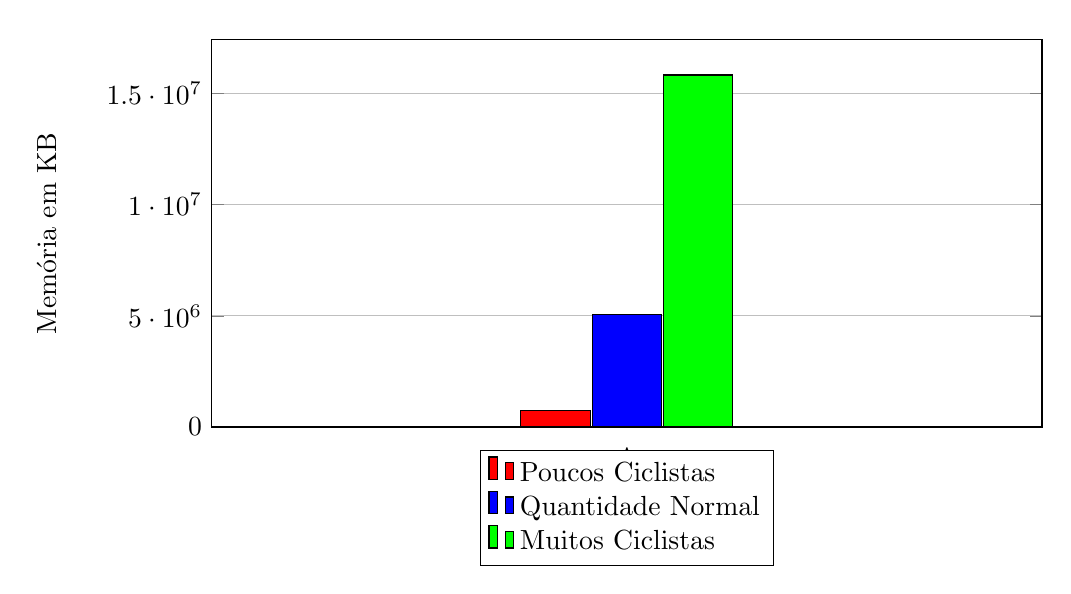
\begin{tikzpicture}
              \begin{axis}[
                  width  = 1.00*\textwidth,
                  height = 6.5cm,
                  major x tick style = transparent,
                  ybar=2*\pgflinewidth,
                  bar width=25pt,
                  ymajorgrids = true,
                  symbolic x coords={A},
                  xtick = data,
                  scaled y ticks = false,
                  enlarge x limits=0.50,
                  ymin=0,
                  ylabel={Memória em KB},
                  ylabel style={yshift=0.4cm},
                  legend cell align=left,
                  legend style={at={(0.5,-0.06)},anchor=north},
              ]

              \addplot[style={fill=red},
                error bars/.cd,
                y dir=both,
                y explicit]
              coordinates {
                (A, 741418)
              };

              \addplot[style={fill=blue},
                error bars/.cd,
                y dir=both,
                y explicit]
              coordinates {
                (A, 5061693)
              };

              \addplot[style={fill=green},
                error bars/.cd,
                y dir=both,
                y explicit]
              coordinates {
                (A, 15824384)
              };

              \legend{Poucos Ciclistas, Quantidade Normal, Muitos Ciclistas}

            \end{axis}
        \end{tikzpicture}
    \end{frame}

    \begin{frame}{Conclusões - Memória}
      \begin{itemize}
        \justifying
        \item Pelos resultados, observamos que o uso de memória não varia com
          alterações no tamanho da pista. Isso era esperado, pois a pista é
          alocada estaticamente e nenhuma memória extra é utilizada quando
          aumentamos o seu tamanho;
        \item Já nos aumentos da quantidade de ciclistas, o uso de memória
          aumentou drasticamente, mas foi um valor igual para todos os 30 testes
          de cada quantidade. Nós esperávamos que houvessem mudanças, pois
          alocamos as listas ligadas dinamicamente de acordo com os
          classificados de cada volta e os ciclistas que quebram (o que não é
          igual em cada teste).
      \end{itemize}
    \end{frame}

    \begin{frame}{Conclusões - Tempo}
      \begin{itemize}
        \justifying
        \item Observamos aumento do tempo tanto ao aumentar o número de
          ciclistas como ao aumentar a pista;
        \item O aumento do número de ciclistas impactou muito mais o tempo de
          execução do que o da pista.
      \end{itemize}
        \textbf{Obs.:} No slide~\ref{segs}, o tempo médio para poucos
          ciclistas foi de $0.5$ segundos com intervalo de confiança de $0.29$
          segundos. Por conta disso, não foi possível a visualização no gráfico.
    \end{frame}

    \begin{frame}
        \centering
        {\huge Obrigado!}

        $\\$

        Lucas e Marcos

    \end{frame}
\end{document}
